% Paquets généraux
\documentclass[a4paper,12pt,titlepage,twoside]{article}
\usepackage[T1]{fontenc}
\usepackage[utf8]{inputenc}
\usepackage[french]{babel}
\usepackage{subcaption}
\addto\captionsfrench{%
  \renewcommand{\tablename}{Tableau}%
}
\usepackage[gen]{eurosym}
%\usepackage[dvips]{graphicx}
\usepackage{minted}
\usepackage{fancyhdr}
\usepackage{pdfpages} 
\usepackage{multido}
\usepackage{hyperref}
\usepackage{textcomp}
\usepackage{schemabloc}
%\usepackage[bitstream-charter]{mathdesign}
\usepackage{array}
\newcolumntype{P}[1]{>{\centering\arraybackslash}p{#1}}
\usepackage[shortlabels]{enumitem}
\usepackage[framemethod=TikZ]{mdframed}

\newcommand{\id}{71}
\newcommand{\nom}{Théorie des mécanismes}
\newcommand{\sequence}{04}
\newcommand{\nomsequence}{Liaisons entre les solides}
\newcommand{\num}{02}
\newcommand{\type}{KH}
\newcommand{\descrip}{Liaisons équivalentes, hyperstatisme, liaisons en série et en parallèle, théorie des graphes}
\newcommand{\competences}{B2-12: Proposer une modélisation des liaisons avec leurs caractéristiques géométriques. \\ &  B2-13: Proposer un modèle cinématique paramétré à partir d'un système réel, d'une maquette numérique ou d'u \\ &  B2-17: Simplifier un modèle de mécanisme. \\ &  B2-18: Modifier un modèle pour le rendre isostatique. \\ &  C1-04: Proposer une démarche permettant d'obtenir une loi entrée-sortie géométrique.  \\ &  C2-05: Caractériser le mouvement d'un repère par rapport à un autre repère. \\ &  C2-06: Déterminer les relations entre les grandeurs géométriques ou cinématiques. }
\newcommand{\nbcomp}{7}
\newcommand{\systemes}{}
\newcommand{\systemesnum}{}
\newcommand{\systemessansaccent}{}
\newcommand{\ilot}{2}
\newcommand{\ilotstr}{02}
\newcommand{\dossierilot}{\detokenize{Ilot_02 }}

%\usepackage{style}
\usepackage{bodegraph}
\usepackage{rpcinematik}
\usepackage[locale = FR]{siunitx}
\usepackage{caption}
\newcommand{\institute}{Lycée Dorian}

\usepackage{listings}
\usepackage{fancyvrb}
\usepackage{color}
\usepackage{xcolor}
\usepackage{colortbl}
\usepackage{helvet}
\usepackage[frenchmath]{newtxsf} % for sans serif symbols
\renewcommand{\familydefault}{\sfdefault}
%\usepackage{amsfonts}
%\usepackage{amsmath}
%\usepackage{lmodern}
\usepackage{mathastext}
%\usepackage{xspace}
\usepackage{varioref}
\usepackage{tabularx}
%\usepackage{floatflt}
\usepackage{graphics}
\usepackage{wrapfig}
\usepackage{textcomp}
\usepackage{tikz,tkz-tab}
\usepackage[european resistor, european voltage, european current]{circuitikz}
\usepackage{wrapfig}
\usepackage{gensymb}
\usepackage[percent]{overpic}
\usetikzlibrary{babel}
\usepackage{ifthen}
\usepackage{cancel}
\usepackage{etoolbox}
\usepackage{multirow}
%\usepackage{boxedminipage}
\definecolor{gris25}{gray}{0.75}
\definecolor{bleu}{RGB}{18,33,98}
\definecolor{bleuf}{RGB}{42,94,171}
\definecolor{bleuc}{RGB}{231,239,247}
\definecolor{bleum}{RGB}{160,195,226}
\definecolor{rougef}{RGB}{185,18,27}
\definecolor{rougec}{RGB}{255,188,204}%255,230,231
\definecolor{vertf}{RGB}{103,126,82}
\definecolor{vertc}{RGB}{220,255,191}
\definecolor{forestgreen}{rgb}{0.13,0.54,0.13}
\definecolor{blcr}{rgb}{0.59,0.69,0.84}
\definecolor{blfr}{rgb}{0.32,0.51,0.75}
\definecolor{orfr}{rgb}{0.90,0.42,0.15}
\definecolor{orcr}{rgb}{0.90,0.65,0.50}
\definecolor{orangef}{rgb}{0.659,0.269,0.072}
\definecolor{orange}{rgb}{0.58,0.35,0.063}
\definecolor{orangec}{rgb}{0.43,0.32,0.25}
\definecolor{rcorrect}{rgb}{0.6,0,0}
\definecolor{sequence}{rgb}{0.75,0.75,0.75}
\definecolor{competences}{rgb}{0.61,0.73,0.35}
\definecolor{rose}{HTML}{ff00ff}
\definecolor{grisf}{HTML}{222222}
\definecolor{grisc}{HTML}{636363}
\definecolor{normal}{HTML}{4087c4}
\definecolor{info}{HTML}{5bc0de}
\definecolor{success}{RGB}{92,184,92}
\definecolor{warning}{RGB}{240,173,78}
\definecolor{danger}{RGB}{217,83,79}
\hypersetup{                    % parametrage des hyperliens
    colorlinks=true,                % colorise les liens
    breaklinks=true,                % permet les retours à la ligne pour les liens trop longs
    urlcolor= blfr,                 % couleur des hyperliens
    linkcolor= orange,                % couleur des liens internes aux documents (index, figures, tableaux, equations,...)
    citecolor= forestgreen                % couleur des liens vers les references bibliographiques
    }

\newcolumntype{M}[1]{>{\centering\arraybackslash}m{#1}}
\definecolor{codegreen}{rgb}{0,0.6,0}
\definecolor{codegray}{rgb}{0.5,0.5,0.5}
\definecolor{codepurple}{rgb}{0.58,0,0.82}
\definecolor{backcolour}{rgb}{0.95,0.95,0.92}

\lstdefinestyle{mystyle}{
    backgroundcolor=\color{backcolour},   
    commentstyle=\color{codegreen},
    keywordstyle=\color{magenta},
    numberstyle=\tiny\color{codegray},
    stringstyle=\color{codepurple},
    basicstyle=\ttfamily\footnotesize,
    breakatwhitespace=false,         
    breaklines=true,                 
    captionpos=b,                    
    keepspaces=true,                 
    numbers=left,                    
    numbersep=5pt,                  
    showspaces=false,                
    showstringspaces=false,
    showtabs=false,                  
    tabsize=2
}

\lstset{style=mystyle}

% Mise en page
\pagestyle{fancy}

\setlength{\hoffset}{-18pt}
\setlength{\oddsidemargin}{0pt} 	% Marge gauche sur pages impaire2s
\setlength{\evensidemargin}{0pt} 	% Marge gauche sur pages paires
\setlength{\marginparwidth}{00pt} 	% Largeur de note dans la marge
\setlength{\headwidth}{481pt} 	 	% Largeur de la zone de tête (17cm)
\setlength{\textwidth}{481pt} 	 	% Largeu\textbf{r de la zone de texte (17cm)
\setlength{\voffset}{-18pt} 		% Bon pour DOS
\setlength{\marginparsep}{7pt}	 	% Séparation de la marge
\setlength{\topmargin}{-30pt} 		% Pas de marge en haut
\setlength{\headheight}{55pt} 		% Haut de page
\setlength{\headsep}{20pt} 		% Entre le haut de page et le texte
\setlength{\footskip}{30pt} 		% Bas de\textbf{ page + séparation
\setlength{\textheight}{700pt} 		% Hauteur de l'icone zone de texte (25cm)
\setlength\fboxrule{1 pt}
\renewcommand{\baselinestretch}{1}
\setcounter{tocdepth}{1}
\newcommand{\cadre}[2]
{\fbox{
  \begin{minipage}{#1\linewidth}
   \begin{center}
    #2\\
   \end{center}
  \end{minipage}
 }
}

\newcommand{\repon}[1]
{
~\ \\
\begin{tabular}{|m{\linewidth}|}
 \hline
\multido{}{#1}{\\ \hline}
\end{tabular}
}


\newcommand{\objectif}[1]{
\mdfsetup{%
frametitle={%
\tikz[baseline=(current bounding box.east),outer sep=0pt]
\node[anchor=east,rectangle,fill=bleum]
{\strut Objectif~};}}
\mdfsetup{innertopmargin=10pt,linecolor=bleum,%
linewidth=2pt,topline=true,%
frametitleaboveskip=\dimexpr-\ht\strutbox\relax
}
\begin{mdframed}[]\relax%
#1
\end{mdframed}}


\newcounter{num_quest} \setcounter{num_quest}{0}
\newcounter{num_rep} \setcounter{num_rep}{0}
\newcounter{num_cor} \setcounter{num_cor}{0}

\newcommand{\feuilleDR}[1]{
	\begin{tikzpicture}
		\draw[gray!30](0,0)grid[step=0.5cm](\linewidth,#1);
	\end{tikzpicture}
}

%\newcommand{\question}[1]{\refstepcounter{num_quest}\par
%~\ \\ \parbox[t][][t]{0.15\linewidth}{\textbf{Question \arabic{num_quest}}}\parbox[t][][t]{0.85\linewidth}{#1\label{q\the\value{num_quest}}}\par
%}

\newcommand{\question}[1]{\refstepcounter{num_quest}\par
~\ \\ \textbf{Question \arabic{num_quest} : }#1\label{q\the\value{num_quest}}\par
}

\newcommand{\posetafigure}[3]{
\begin{figure}[ht!]
 \begin{center}
  \includegraphics[width=#2\linewidth]{img/#1}
 \end{center}
 \caption{\label{#1} #3}
\end{figure}}

\newcommand{\goforum}{
\begin{figure}

\end{figure}
\begin{center}
 
\includegraphics[width=0.7\linewidth]{../../../img/go_forum}
\end{center}
\label{go_forum}
\caption{J'pète les plombs}
\end{figure}}

\newcommand{\reponse}[4][1]
{\noindent
\parbox{\textwidth}{
\rule{\linewidth}{.5pt}\\
\textbf{Question\ifthenelse{#1>1}{s}{} \multido{}{#1}{%
\refstepcounter{num_rep}\ref{q\the\value{num_rep}} }:} ~\ \\
\ifdef{\public}{#3 \ifthenelse{#2>0}{~\ \\ 	\feuilleDR{#2}}}{#4}
}}

\newcommand{\cor}
{\refstepcounter{num_cor}
\noindent
\rule{\linewidth}{.5pt}
\textbf{Question \arabic{num_cor}:} \\
}

\newcommand{\finsujet}
{
    \begin{center}
    \Large{FIN}
    \end{center}

    \cleardoublepage

    \ifdef{\public}{\pagestyle{docreponse}}{\pagestyle{correction}}

    \ifdef{\public}{
        \begin{tikzpicture} 
            \draw (0,0) rectangle (2,2);
            \draw (0,0) -- (2,2);
            \draw (1.5,0.5) node {\large 20};
            \draw (2.5,0) rectangle (16,2);
            \draw (4.5,1.7) node {\large Commentaires:};
        \end{tikzpicture}
    }
    ~\ \\
}


%\newcommand{\repcarre}[2]
%{
%~\ \\
%\begin{tikzpicture}
%\draw [fill=white] (0,0) rectangle +(\linewidth,#1);
%\node[align=left] at (1.1,#2-0.3) {\textbf{Question #1:}};
%\end{tikzpicture}
%}

\newcommand{\titre}[1]
{\begin{center}
\cadre{0.8}{\huge #1} 
\end{center}
}


%Définition des torseurs :
\newcommand{\torseur}[2]{\left\{\mathcal{#1}_{#2} \right\}}
\newcommand{\torseurh}[3]{\left\{\genfrac{}{}{0pt}{0}{#1}{#2}\right\}_{#3}}
\newcommand{\torseurv}[8]{\left\{
\begin{matrix}
#1 & #4 \\ #2 & #5 \\ #3 &#6
\end{matrix}
\right\}_{{#7},{#8}}}

%Définition des torseurs :
%\newcommand{\torseur}[2]{\left \{\mbox{\relsize{2}{$\mathcal {#1}$}\relsize{-2}}\phantom{}_{\mbox{\scriptsize $#2$}} \right \}}
%\newcommand{\torseurh}[3]{\left\{\genfrac{}{}{0pt}{0}{#1}{#2}\right\}_{#3}}
%\newcommand{\torseurv}[8]{
%\left\{\begin{array}{@{}c|c@{}} #1 & #4 \\ #2 & #5 \\ #3 & #6 \end{array} \right\}_{#7,#8}
%}
\newcommand{\derivee}[2]{\left.\dfrac{\d #1}{\d t}\right|_{#2}}
\newcommand{\tripleint}{\int\!\!\!\!\!\int\!\!\!\!\!\int}

% Notation cinématique et statique
\newcommand{\cinematique}[2]{\mbox{#1}/\mbox{#2}}
\newcommand{\statique}[2]{\mbox{#1}\rightarrow\mbox{#2}}
\newcommand{\moment}[3]{\vv {#1}_{\scriptsize{#3}}(#2)}
\newcommand{\resultante}[2]{\vv {#1}_{\scriptsize{#2}}}


%Commande de base
\newcommand{\jo}{\left(j\omega\right)} % j \omega dans l'analyse fréquentielle
\newcommand{\tl}{\xrightarrow{\mathcal{L}}} % transformée de laplace sur fleche
\newcommand{\tli}{\xrightarrow{\mathcal{L}^{-1}}} % transformée inverse de laplace sur fleche
\renewcommand{\d}[1][]{\mathrm{d#1}}
\newcommand{\dd}[1][]{\mathrm{d#1}}
\newcommand{\vect}[2]{{#1}\wedge{#2}}
\newcommand{\base}[3]{(\vec #1,\vec #2,\vec #3)}
\newcommand{\vectbase}[4]{{\vphantom{\left| \begin{matrix}
#1\\#2\\#3 \end{matrix} \right|}}_{#4}{\left| \begin{matrix}
#1\\#2\\#3 \end{matrix} \right.}}
%Pour avoir les paragraphes sous la forme I, II, III
\renewcommand{\thesection}{\Roman{section}}
\setcounter{secnumdepth}{3}
\renewcommand{\Frlabelitemii}{$\bullet$}

% En tête et pied de page
\lhead{\nom}
\rhead{
\includegraphics[width=2cm]{../../../img/logo}}
\lfoot{\auteurun,\ \auteurdeux}
\cfoot{Page \thepage}

\fancypagestyle{docreponse}{%
  \fancyhf{}
  \fancyhead[LO]{NOM Prénom: .............................}
  \rhead{
\includegraphics[width=2cm]{../../../img/logo}\hspace{2pt}}
  \ifdef{\auteurdeux}{\lfoot{\auteurun,\ \auteurdeux}}{\lfoot{\auteurun}}
  \rfoot{\nom}
  \lfoot{Document réponse}
  \cfoot{Page \thepage}
   }

\fancypagestyle{correction}{%
  \fancyhf{}
  \lhead{\colorbox{danger}{\begin{minipage}{0.65\paperwidth} \textcolor{white}{\textbf{Correction}} \end{minipage}} }
  \rhead{
\includegraphics[width=2cm]{../../../img/logo}}
  \lfoot{Renaud Costadoat, Françoise Puig}
  \rfoot{\colorbox{danger}{\begin{minipage}{0.4\paperwidth} \begin{flushright}\textcolor{white}{\textbf{Correction}}\end{flushright} \end{minipage}} }}

\fancypagestyle{correctioninfo}{%
  \fancyhf{}
  \lhead{\colorbox{danger}{\begin{minipage}{0.65\paperwidth} \textcolor{white}{\textbf{Correction}} \end{minipage}} }
  \rhead{
\includegraphics[width=2cm]{../../../img/logo}}
  \lfoot{Renaud Costadoat, Juliette Genzmer}
  \rfoot{\colorbox{danger}{\begin{minipage}{0.6\paperwidth} \begin{flushright}\textcolor{white}{\textbf{Correction}}\end{flushright} \end{minipage}} }}

\renewcommand{\footrulewidth}{0.4pt}

\usepackage{eso-pic}
\newcommand{\BackgroundPic}{%
\put(0,0){%
\parbox[b][\paperheight]{\paperwidth}{%
\vfill
\begin{center}
\hspace{0.5cm}\vspace{0.5cm}

\includegraphics[width=\paperwidth,height=\paperheight,%
keepaspectratio]{../../../img/fond3}%
\end{center}
\vfill
}}}

\newcommand{\BackgroundPicdeux}{%
\put(25,-30){%
\parbox[b][\paperheight]{\paperwidth}{%
\vfill
\begin{center}

\includegraphics[width=\paperwidth,height=\paperheight,%
keepaspectratio]{../../../img/fond4}%
\end{center}
\vfill
}}}

\begin{document}

\pagestyle{empty}

\AddToShipoutPicture*{\BackgroundPic}


\includegraphics[width=2cm]{../../../img/logo}

\Huge{DS \numero - \sujet}

\vspace{1cm}

\ifdef{\prive}{\begin{center}\colorbox{danger}{\Huge{Avec Correction}}\end{center}}{}

\begin{center}
\centering\huge{PTSI}
\end{center}

\vspace{2cm}


\begin{center}
\centering\Large{\jour}
\end{center}

\vspace{2cm}

\normalsize

\tableofcontents

\newpage

\AddToShipoutPicture{\BackgroundPicdeux}

\pagestyle{fancy}

\begin{center}
\Huge \sujet
\end{center}


\normalsize


\section{Présentation du système \og Robot de traite automatique \fg}

\subsection{Contexte}

Les agriculteurs, producteurs laitiers, sont soumis à des réglementations strictes quant à la production du lait, en termes de respect de l’environnement, de mesures d’hygiène et de qualité de vie des animaux.

Traire les vaches est une opération pénible et répétitive. Cette opération doit se faire dans le respect des animaux et elle est soumise à des horaires contraignants. Les agriculteurs souhaitent maintenant disposer de plus de temps pour gérer leur exploitation agricole et pouvoir concilier vie professionnelle et personnelle. Dans cette optique, des sociétés ont développé des systèmes de traite automatique.

Le robot à étudier améliore de façon notable la santé et la qualité de vie des producteurs laitiers, tout en préservant le rythme des animaux et en garantissant la qualité du lait. Il assure à la fois la traite des vaches, leur alimentation et le contrôle de la qualité du lait (en identifiant les éventuels problèmes de santé, en mesurant les paramètres essentiels, en détectant le lait non conforme).

\begin{figure}[ht!]
\begin{center}
 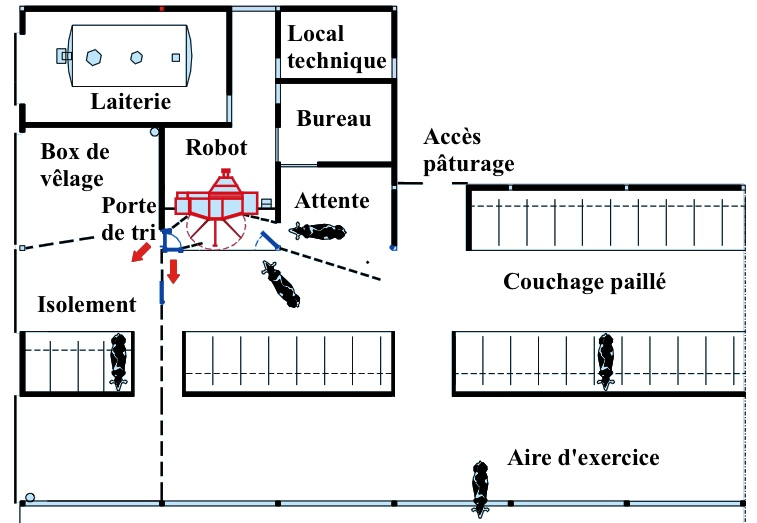
\includegraphics[width=0.6\linewidth]{img/fig001}
\end{center}
\label{fig001}
\caption{Exemple d'implantation du robot de traite dans une exploitation agricole}
\end{figure}

\subsection{Description du robot de traite}

\begin{figure}[ht!]
\begin{center}
 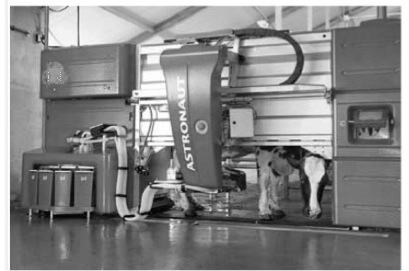
\includegraphics[width=0.4\linewidth]{img/fig002}
\end{center}
\label{fig002}
\caption{Robot de traite Lely}
\end{figure}

\begin{figure}[ht!]
\begin{center}
 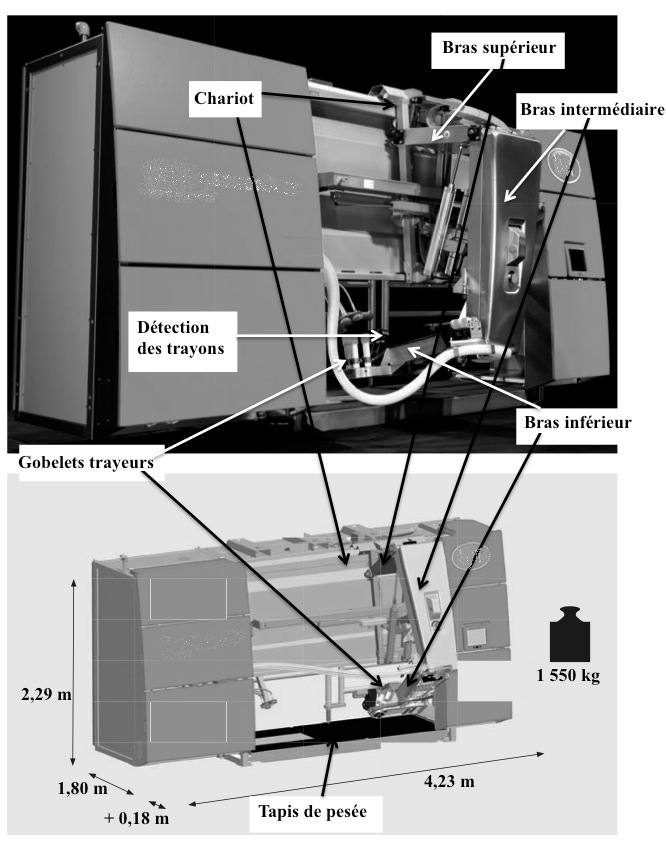
\includegraphics[width=0.5\linewidth]{img/fig003}
\end{center}
\label{fig003}
\caption{Description des composants principaux du robot de traite Lely}
\end{figure}

Le robot Lely est composé (figure \ref{fig003}) :
\begin{itemize}
 \item d’une zone (box où la vache est installée lors de la traite) composée d’une structure tubulaire mécanosoudée, équipée de 2 portes (entrée et sortie), d’un tapis de pesée et d’une auge réservée à l’alimentation solide (granulés) ;
 \item d’un système de bras articulé, permettant au système de traite de se positionner au mieux pour traire la vache ;
 \item d’une interface homme/machine, écran de contrôle tactile, qui permet au personnel agricole d’obtenir des renseignements sur le processus en cours et de gérer d’éventuelles opérations de maintenance.
\end{itemize}

Le bras articulé se décompose en 2 parties :
\begin{itemize}
 \item le chariot, permettant le déplacement horizontal du bras. Il est monté sur des galets qui réalisent la liaison glissière de direction horizontale et un vérin pneumatique commande le déplacement de ce chariot. Le système de contrôle du bras est installé sur le chariot ;
 \item le bras, composé :
 \begin{itemize}
  \item d’un bras supérieur en liaison pivot d’axe horizontal par rapport au chariot. Deux vérins montés en parallèle entre le chariot et le bras supérieur assurent les déplacements de ce dernier;
  \item d’un bras intermédiaire, lié au bras supérieur par une liaison pivot. Un vérin monté entre le bras intermédiaire et le chariot assure les déplacements du bras intermédiaire ;
  \item d’un bras inférieur, en liaison complète avec le bras intermédiaire, qui porte le système de branchement aux trayons (ou mamelles, ou pis), le système pulsateur, le système de nettoyage par brosses (en liaison pivot avec le bras inférieur) et la tête de traite ;
  \item d’une tête de traite, constituée des gobelets et du système de détection des trayons de la vache (le système TDS utilise une technologie laser en trois dimensions pour un repérage rapide et précis des trayons, permettant le positionnement et le branchement rapide des gobelets).
\end{itemize}
\end{itemize}

\subsection{Description d’une traite automatique}

Le principe de la traite automatique est de laisser la vache libre de choisir le moment où elle souhaite être traite.

Toutes les vaches laitières du troupeau sont équipées d’un collier d’identification à infrarouge qu’elles portent autour du cou.

Lorsqu’elle le décide, la vache se présente devant la porte d’entrée du box de traite. Grâce à son collier, elle est identifiée (les informations sont gérées par un ordinateur superviseur).

La porte d’entrée s’ouvre, laissant passer la vache (et elle seule), puis se referme. La vache est alors isolée dans le box de traite. Elle se dirige naturellement vers l’auge pour manger sa ration de granulés. Grâce aux informations d’identification, la nourriture est dosée.

\begin{itemize}
 \item Cas 1 : si la vache a déjà été traite récemment et ne respecte pas le temps minimum entre 2 traites, aucun aliment ne sera distribué. Elle ne sera pas traite, la porte de sortie sera alors ouverte, laissant sortir l’animal et libérant le box de traite.
 \item Cas 2 : si la vache a respecté le temps entre 2 traites et qu’elle n’a pas eu sa dose journalière de granulés, l’auge sera alors remplie avec la dose adéquate de granulés.
\end{itemize} 

Lorsque la vache est dans le box, elle est installée sur un tapis de pesée équipé de capteurs de pesage. Les informations de masse et de position du centre de gravité de l’animal sont transmises à l’ordinateur superviseur. Le bras du robot peut alors être positionné et effectuer la traite de la vache.

Connaissant le centre de gravité de la vache, le bras vient positionner le bras inférieur (avec la tête de traite) au plus près des trayons de la vache. Le système de nettoyage par brosses vient alors se positionner au niveau des trayons de la vache, nettoyant trayon par trayon et stimulant la lactation (venue du lait). Une fois cette tâche effectuée, le système se retire (système escamotable, en liaison pivot avec le bras inférieur).

Ensuite, le système de triangulation laser permet de positionner les gobelets trayeurs un par un, toujours dans le même ordre : il détecte la position du premier trayon, puis positionne le premier gobelet trayeur, puis il détecte la position du second trayon et positionne le deuxième gobelet trayeur et idem pour les troisième et quatrième gobelets trayeur. Dès qu’un gobelet trayeur est « branché » sur le trayon, un système pulsateur s’enclenche et tire le lait qui est acheminé vers une chambre de réception (qui stockera tout le lait de cette vache, permettant ainsi de connaître la quantité de lait extrait lors de la traite, informant alors l’ordinateur). Lorsque tous les trayons sont branchés, le système de nettoyage (brosses) est nettoyé.

Lorsque le système pulsateur détecte une absence de lait dans un trayon, le gobelet trayeur est alors déconnecté (chaque gobelet trayeur est déconnecté de façon indépendante). Lorsque les 4 gobelets sont déconnectés, les trayons de la vache sont nettoyés (par aspersion d’eau).

Le bras se retire, les gobelets trayeurs sont nettoyés à la vapeur puis rincés à l’eau claire. Le lait qui était dans la chambre de réception est pesé s’il est « sain » puis acheminé vers le tank à lait par un lactoduc (figure 4). S’il n’est pas « sain », il est acheminé directement vers les égouts. Dans tous les cas, la chambre est ensuite nettoyée de façon à ne pas contaminer le lait de la prochaine vache.

La traite est alors terminée. La porte de sortie s’ouvre, incitant la vache à quitter le box de traite.

\begin{figure}[ht!]
\begin{center}
 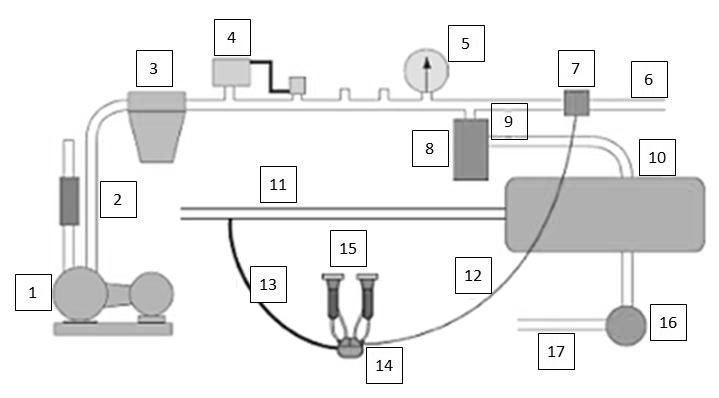
\includegraphics[width=0.6\linewidth]{img/fig004}
\end{center}
\label{fig004}
\caption{Principaux composants du système de traite avec lactoduc}
\end{figure}

\begin{minipage}[t]{0.52\linewidth}
\begin{enumerate}
\item Pompe à vide
\item Canalisation principale (air)
\item Intercepteur
\item Régulateur
\item Indicateur de vide
\item Canalisation à air des pulsateurs
\item Pulsateur
\item Piège sanitaire
\item Canalisation à air de la chambre de réception
\end{enumerate}
\end{minipage}
\hfill
\begin{minipage}[t]{0.45\linewidth}
\begin{enumerate}
\setcounter{enumi}{9}
\item Chambre de réception
\item Lactoduc
\item Tuyau long de pulsation
\item Tuyau long à lait
\item Griffe
\item Gobelet trayeurs
\item Pompe à lait
\item Lactoduc d’évacuation
\end{enumerate}
\end{minipage}


\section{Implantation dans une exploitation agricole du \og Robot de traite automatique \fg}

\paragraph{Objectif :} valider la pertinence de l’implantation d’un seul robot dans une exploitation agricole ayant 60 vaches laitières.

Le robot de traite Lely est prévu pour fonctionner 20 heures sur 24 : sur cette durée, la moyenne sur le troupeau est de 2,5 traites par vache, la durée moyenne d’une traite étant de 6 minutes.

Par ailleurs, afin d’assurer une hygiène parfaite, des nettoyages réguliers sont prévus et, lors de ces opérations, le box n’est pas accessible. Deux types de nettoyage sont réalisés :
\begin{itemize}
 \item des nettoyages simples à l’eau chaude des parties en contact avec le lait (gobelets, etc.) qui durent 4 minutes et sont exécutés toutes les 5 traites ;
 \item et des nettoyages complets de l’ensemble du robot qui durent 10 minutes et sont exécutés toutes les 20 traites et aussi après les 20 heures de fonctionnement, quel que soit le nombre de traites effectuées.   
\end{itemize}

Un cycle de traites correspond au temps séparant deux nettoyages complets.

\question{Déterminer la durée d’un cycle de traites $d_t$.}

\question{Déterminer le nombre entier $n$ de cycles de traites quotidiennement effectués par le robot dans les conditions de fonctionnement définies.}

\question{Déterminer le temps $t_d$ restant disponible et en déduire le nombre de traites complémentaires possibles.}

\question{En déduire le nombre total de traites $n_t$ que peut effectuer le robot sur une plage d’utilisation de 20 heures.}

\question{Définir alors la taille maximale $t_{max}$ du troupeau pour un seul robot Lely. Est-ce compatible avec le cheptel de 60 vaches de l’entreprise agricole ?}

\section{Analyse fonctionnelle du système \og Robot de traite automatique \fg}

\subsection{Exigences du système étudié}

Grâce à la traite automatique, les vaches choisissent leurs heures de traite et se déplacent librement entre le robot de traite et les bâtiments d’élevage. Les éleveurs n’ont alors plus de contraintes horaires fixes de traite, ce qui leur permet de gérer au mieux leur exploitation agricole.

En annexe (fin du sujet), on fournit les diagrammes des exigences du système étudié.

\question{A l’aide de la description fournie dans la « Partie 1. Présentation du système « Robot de traite automatique » du sujet, et des diagrammes SysML en annexe, compléter le diagramme de contexte sur le document réponse.}

\question{Quelles sont les 2 exigences principales du système « robot de traite automatique » ?}

\subsection{Modules du système étudié}

En annexe (fin du sujet), on fournit un diagramme de définition de bloc du système « robot  Lely ».

\question{Grâce à quel sous-système le robot détecte-il le pis de la vache ?}

\question{Quel composant technique permet d’obtenir l’information de pesée de la vache ?}

\question{Quel composant technique permet d’identifier la vache présente dans le box de traite automatique ?}

\subsection{Peser la vache}

Lorsqu’elle est dans le box, la vache est sur un tapis de pesée, schématisé figure 5. Ce tapis de pesée est constitué d’une structure rigide (caillebotis métallique) liée au support des capteurs (bâti tubulaire mécanosoudé) et d’un revêtement antidérapant en caoutchouc.

\paragraph{Objectif :} on souhaite vérifier que la pesée de la vache soit fournie à 2\% près.

\begin{figure}[ht!]
\begin{center}
 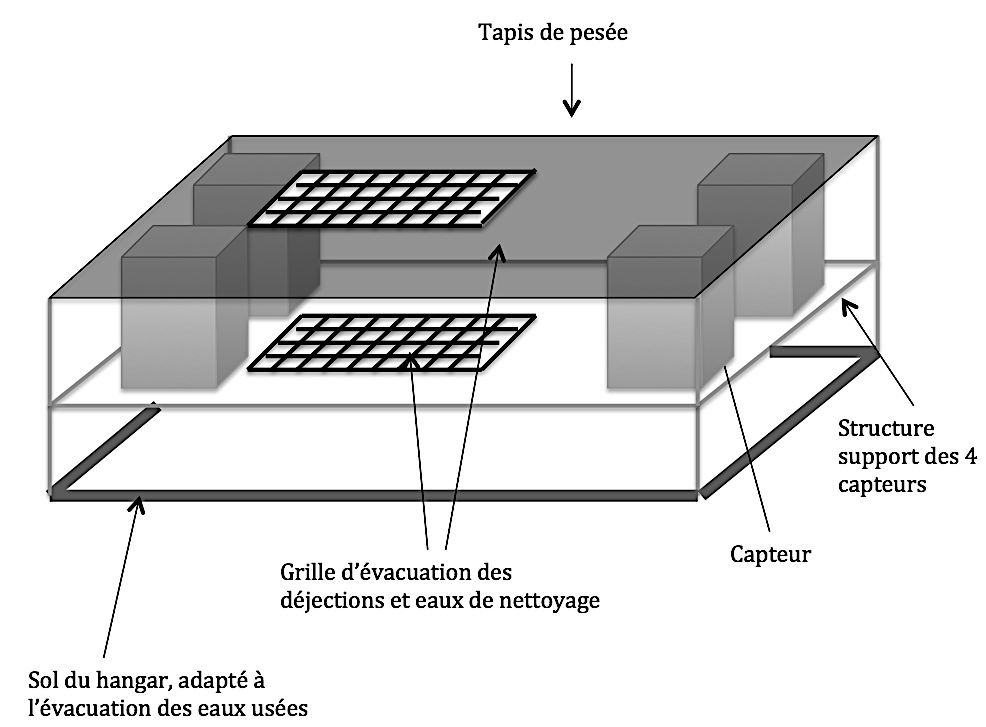
\includegraphics[width=0.6\linewidth]{img/fig005}
\end{center}
\label{fig005}
\caption{Schéma du tapis de pesée et de son implantation}
\end{figure}

\begin{tabular}{|l|l|l|}
\hline
& Dimensions (mm)& Matériau\\
\hline
Revêtement antidérapant & 2500×1000×10 & caoutchouc recyclé (masse volumique: 900 kg/m3) \\
\hline
Structure rigide & 2500×1000×20 & acier galvanisé (masse surfacique: 15 kg/m2)\\
\hline
Grille d’évacuation & 700×500×20 & acier galvanisé (masse surfacique: 15 kg/m2).\\
\hline
\end{tabular}

4 capteurs identiques de pesée à appui central se trouvent sous ce tapis de pesée. Les caractéristiques de ces capteurs sont données dans le tableau suivant :


\begin{minipage}{0.4\linewidth}
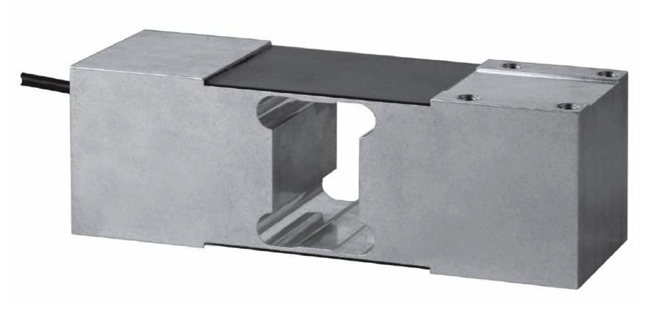
\includegraphics[width=0.9\linewidth]{img/tab001}
\end{minipage}
\begin{minipage}{0.55\linewidth}
\begin{itemize}
 \item Poids, y compris emballage: 2 kg
 \item Applications: Balances sur table, plateforme au sol, convoyage et applications médicales,
 \item Particularités: Gamme étendue de capacités nominales de 30 jusqu’à 750 kg
\end{itemize}
\end{minipage}

\question{Sachant qu’une vache a une masse de 700 kg en moyenne et connaissant les caractéristiques des 4 capteurs utilisés, peut-on négliger la masse du tapis de pesée (structure rigide et revêtement antidérapant) et respecter une précision de pesée de 2\% ?
Vous justifierez vos réponses par le calcul. Quelle(s) opération(s) devra réaliser l’installateur lors de la mise en service du tapis de pesée ?}

\section{Mettre en position le système nécessaire à la traite}

La vache étant identifiée, le robot doit se mettre en position afin de démarrer le cycle de traite.

\subsection{Détecter la position de la vache}

Lorsque la vache arrive sur le tapis de pesée, les informations délivrées par les capteurs permettent non seulement d’avoir l’information de la masse de la vache, mais ils permettent également d’obtenir la position du centre de gravité de la vache.

\begin{figure}[ht!]
\begin{center}
 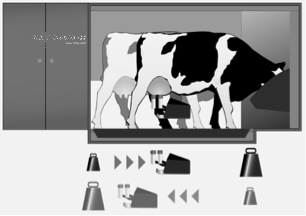
\includegraphics[width=0.6\linewidth]{img/fig006}
\end{center}
\label{fig006}
\caption{Détection de la position de la vache}
\end{figure}

Le système de traite étant positionné au plus proche du pis de la vache nous allons nous intéresser plus particulièrement au mouvement du chariot 1, lorsque le robot est en phase de traite de la vache (gobelets trayeurs positionnés sur la vache et en mode extraction du lait).

\begin{figure}[ht!]
\begin{center}
 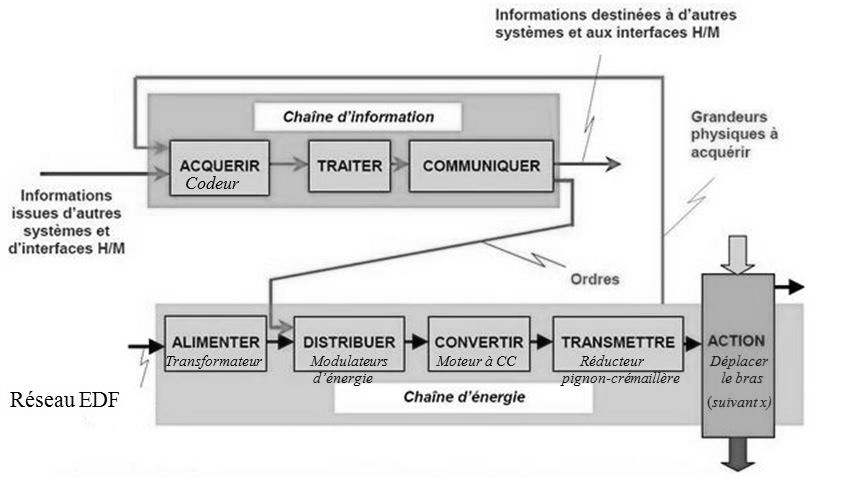
\includegraphics[width=0.8\linewidth]{img/fig007}
\end{center}
\label{fig007}
\caption{Sstructure de l’axe motorisé du chariot}
\end{figure}

\newpage

Données du moteur à courant continu : 
\begin{itemize}
 \item résistance de l’induit : $R=5\Omega$,
 \item inductance : $L=0,0053H$,
 \item constante de fem : $Ke=0,65V.s.rad-1$,
 \item constante de couple $K_i=0,65N.m.A^{-1}$,
 \item coefficient de frottements visqueux dans les liaisons ramené à l'arbre moteur : $\mu=0,001N.s.rad^{-1}$,
\item inertie ramenée à l’arbre moteur : $J=8.10^{-3}kg.m^2$.
\end{itemize}

Les condition initiales sont nulles. On note $U_m(p)=L[u_m(t)]$,$I_m(p)=L[i_m(t)]$,$E(p)=L[e(t)]$,$\Omega_m(p)=L[\omega_m(t)]$,$C_m(p)=L[c_m(t)]$.

\begin{eqnarray}
u_m(t)=R\cdot i_m(t)+L\cdot \frac{di_m(t)}{dt}+e(t) \\
e(t)=K_e\cdot \omega_m(t) \\
c_m(t)=K_c\cdot i_m(t) \\
J.\frac{d\omega_m(t)}{dt}=c_m(t)-\mu.\omega_m(t)
\end{eqnarray}

\question{En utilisant le théorème de la dérivation, écrire les 4 équations du moteur dans le domaine de Laplace.}

\question{Déterminer la fonction de transfert $H(p)=\frac{\Omega_m(p)}{U_m(p)}$.}

\question{Écrire la fonction de transfert $H(p)$ sous la forme $H(p)=\frac{G}{1+\frac{2.\xi}{\omega_n}.p+\frac{2}{\omega_n^2}.p^2}$.}

\question{Donner les expressions du facteur d’amortissement $\xi$, de la pulsation propre $\omega_n$ et le gain $G$ en fonction des paramètres de l’énoncé.}

\question{Donner l’unité de $G$ en unité S.I. de base et faire l’application numérique.}

\question{Faire les applications numériques pour $\omega_n$ et $\xi$, vous préciserez les unités.}

Pour la suite, on prendra $w_n=100$ et $z=5$.

\question{Justifier qu’on peut alors écrire $H(p)$ sous la forme $H(p)=\frac{G}{(1+\tau_1.p)(1+\tau_2.p)}$ et donner les valeurs numériques de $\tau_1$ et$\tau_2$.}

\question{Quelle(s) hypothèse(s) pouvez-vous faire afin d’assimiler $H(p)$ à un premier ordre ? Donner alors la nouvelle expression de $H(p)$ sous forme canonique littérale et l’écrire avec également sous forme numérique.}

Quels que soient les résultats trouvés précédemment, on prend maintenant $H(p)=\frac{1}{1+0,005\cdot p}$.

On sollicite le moteur avec un échelon  $u_0=25 V$.

\question{Déterminer alors l’expression de $\omega_m(t)$.}

On donne les 2 réponses temporelles suivantes : figure \ref{fig008a} et figure \ref{fig008b}.

\begin{figure}[ht!]
  \begin{subfigure}{0.45\textwidth}
    \begin{center}
	 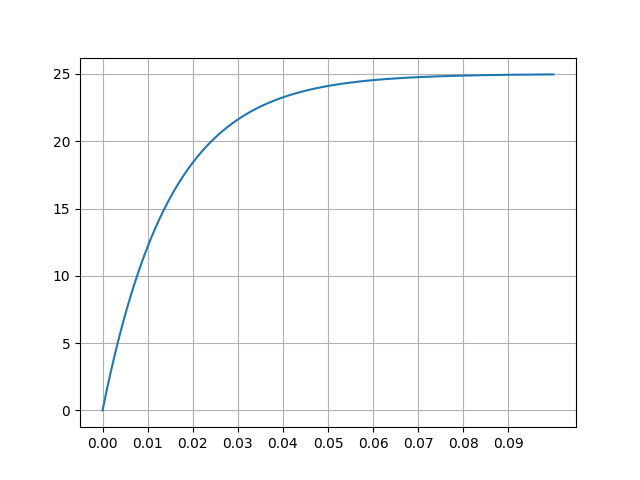
\includegraphics[width=0.9\linewidth]{img/fig008a}
	\end{center}
    \caption{Solution 1} \label{fig008a}
  \end{subfigure}%
  \hspace*{\fill}   % maximize separation between the subfigures
  \begin{subfigure}{0.45\textwidth}
    \begin{center}
	 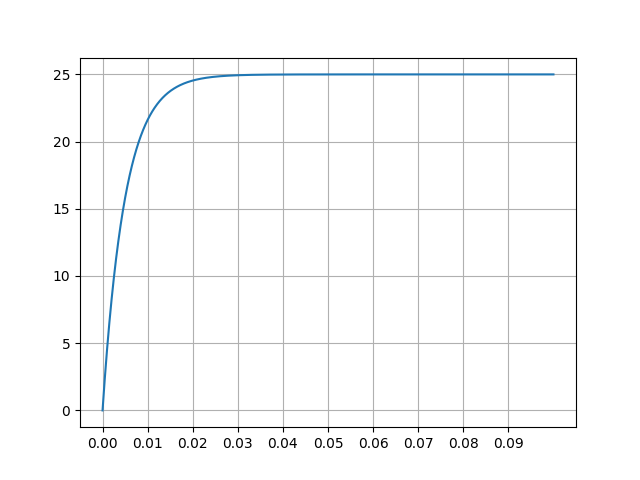
\includegraphics[width=0.9\linewidth]{img/fig008b}
	\end{center}
    \caption{Solution 2} \label{fig008b}
  \end{subfigure}%
\end{figure}
  
\question{Déterminer à laquelle correspond celle calculée à la question Q19. Justifier la réponse en indiquant pour chacune d’elle ce qui la différencie du résultat attendu.}

\newpage

\section{Identification d’une réponse temporelle}

Soit la réponse temporelle $s(t)$ en $rad.s^{-1}$ à un échelon $u_0(t)=12V$.

\begin{figure}[ht!]
\begin{center}
 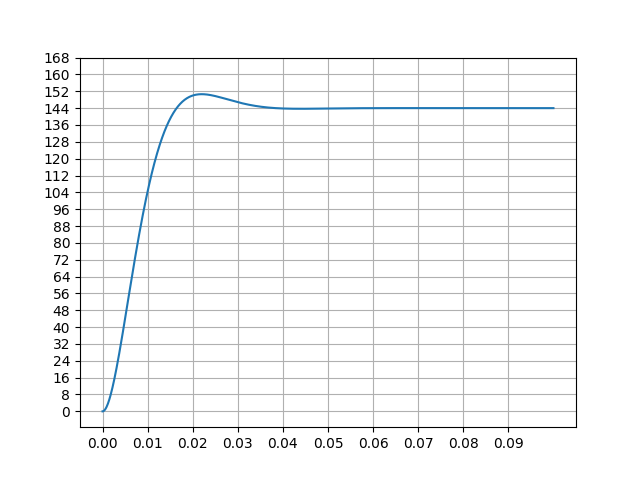
\includegraphics[width=0.6\linewidth]{img/fig009}
\end{center}
\label{fig009}
\caption{Réponse à un échelon $u_0(t)=12V$}
\end{figure}

\question{Déterminer (le gain statique) $K$ de la fonction de transfert correspondante, vous préciserez l’unité.}

\question{Déterminer $\xi$ (à 0,1 près) de la fonction de transfert correspondante, vous préciserez l’unité.}

\question{Déterminer $\omega_0$ de la fonction de transfert correspondante, vous préciserez l’unité.}

\newpage

\section{Annexes}
    
\begin{figure}[ht!]
\begin{center}
 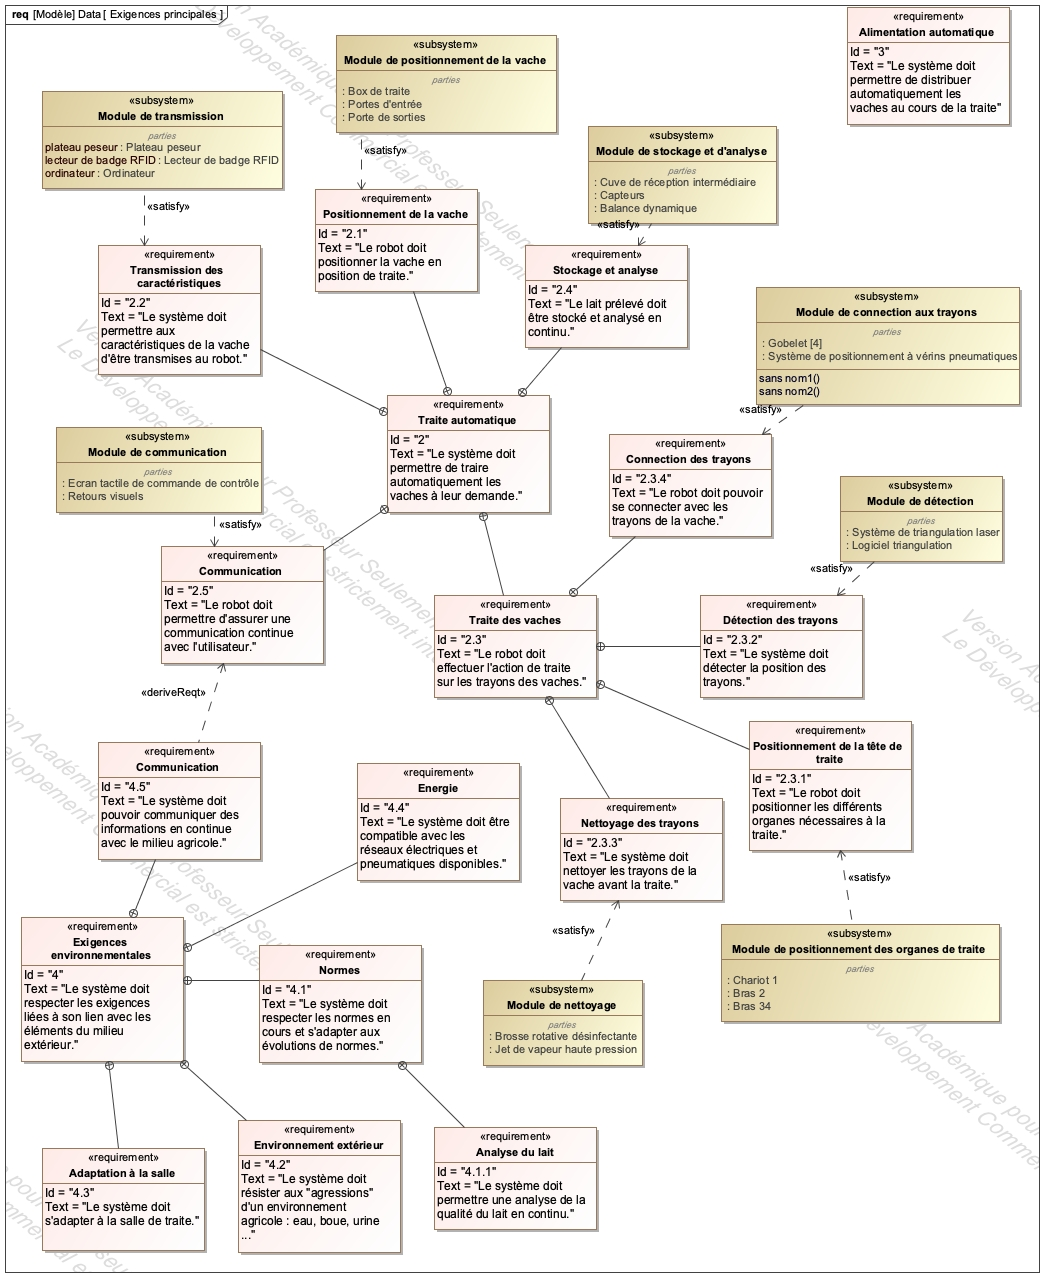
\includegraphics[width=0.9\linewidth]{img/fig010}
\end{center}
\label{fig010}
\caption{Diagramme des exigences 1}
\end{figure}

\newpage

\begin{figure}[ht!]
\begin{center}
 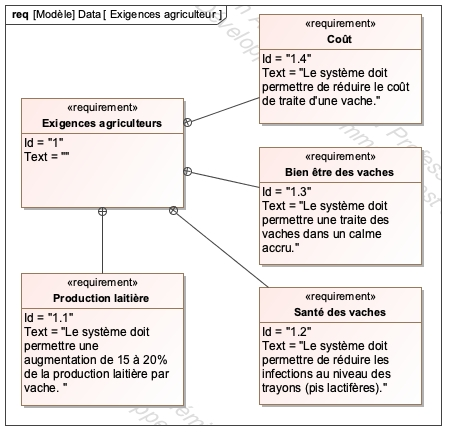
\includegraphics[width=0.6\linewidth]{img/fig011}
\end{center}
\label{fig011}
\caption{Diagramme des exigences 2}
\end{figure}

\newpage

\begin{figure}[ht!]
\begin{center}
 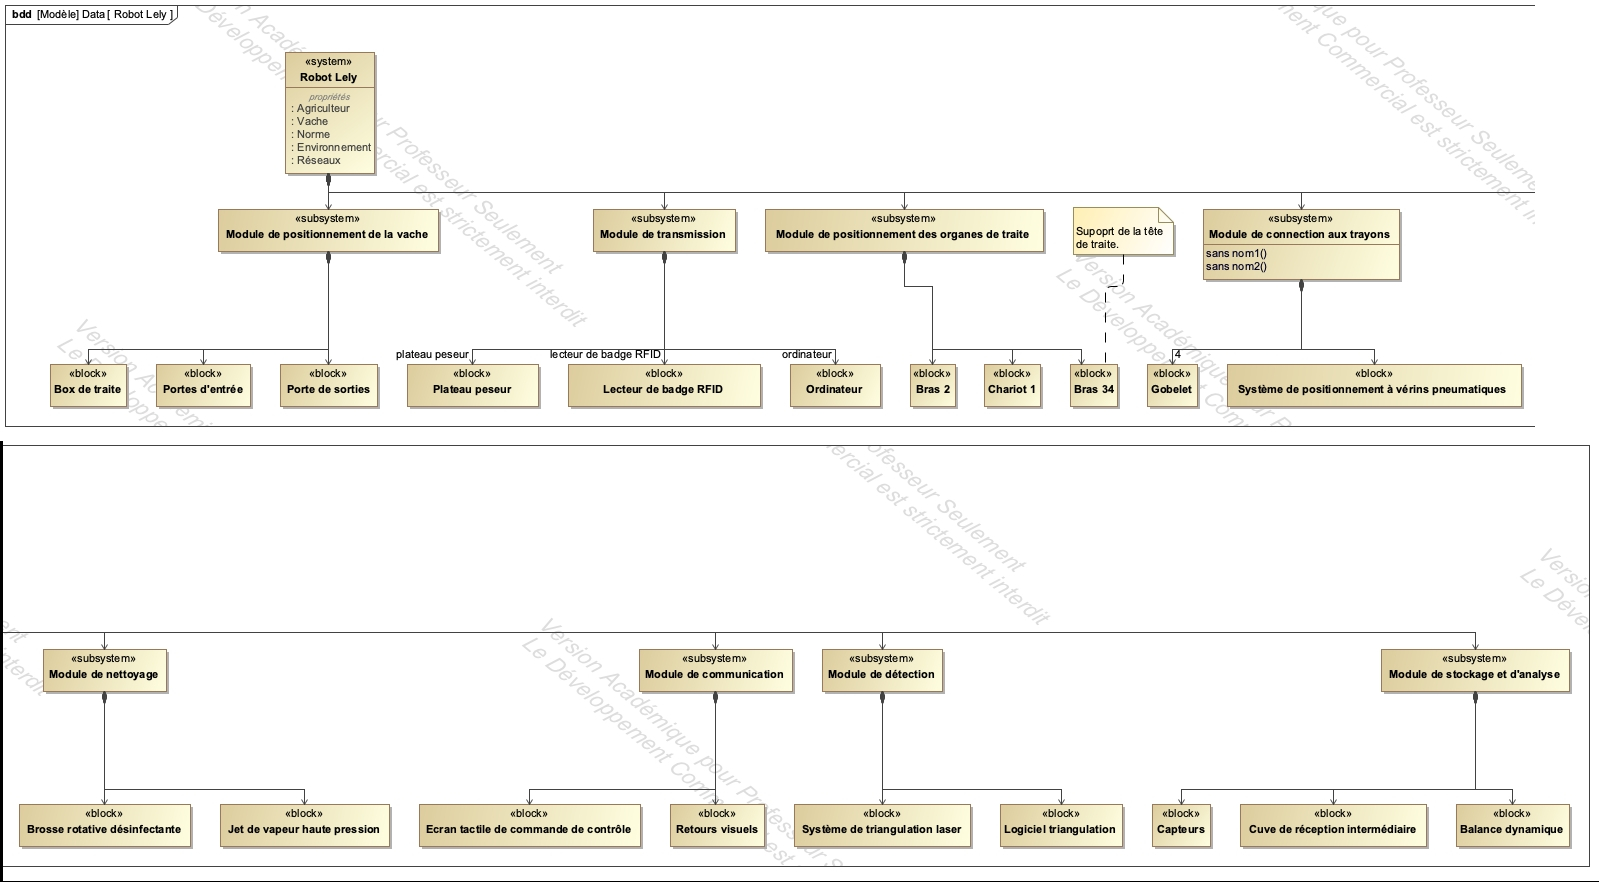
\includegraphics[width=1.4\linewidth,angle=90]{img/fig012}
\end{center}
\label{fig012}
\caption{Diagramme de blocs}
\end{figure}


\cleardoublepage


\ifdef{\public}{\pagestyle{documentreponse}}{\pagestyle{correction}}

\reponse{4}{}{La durée d'un cycle est $d_{cycle}=20\cdot d_t+3\cdot d_{ns}+1\cdot d_{nc}=20\cdot6+3\cdot4+1\cdot 10=120+12+20=142 minutes=2heure22min$.}

\reponse{4}{}{Sur une durée quotidienne de 20h, il est possible de faire $n=\frac{20*60}{142}=\frac{1200}{142}=8cycles$.}

\reponse{4}{}{Il reste alors $t_d=1200-8\cdot 142=1200-800-320-16=64min$.}

\reponse{4}{}{En $64min$, il est possible de faire encore 10 traites. Donc, le total peut être porté à $n_t=8\cdot20+10=170traites$.}

\reponse{4}{}{A raison d'une moyenne de 2,5 traites par vache cela donne pour 1 robot 68 vaches.}

\reponse{4}{\begin{center}
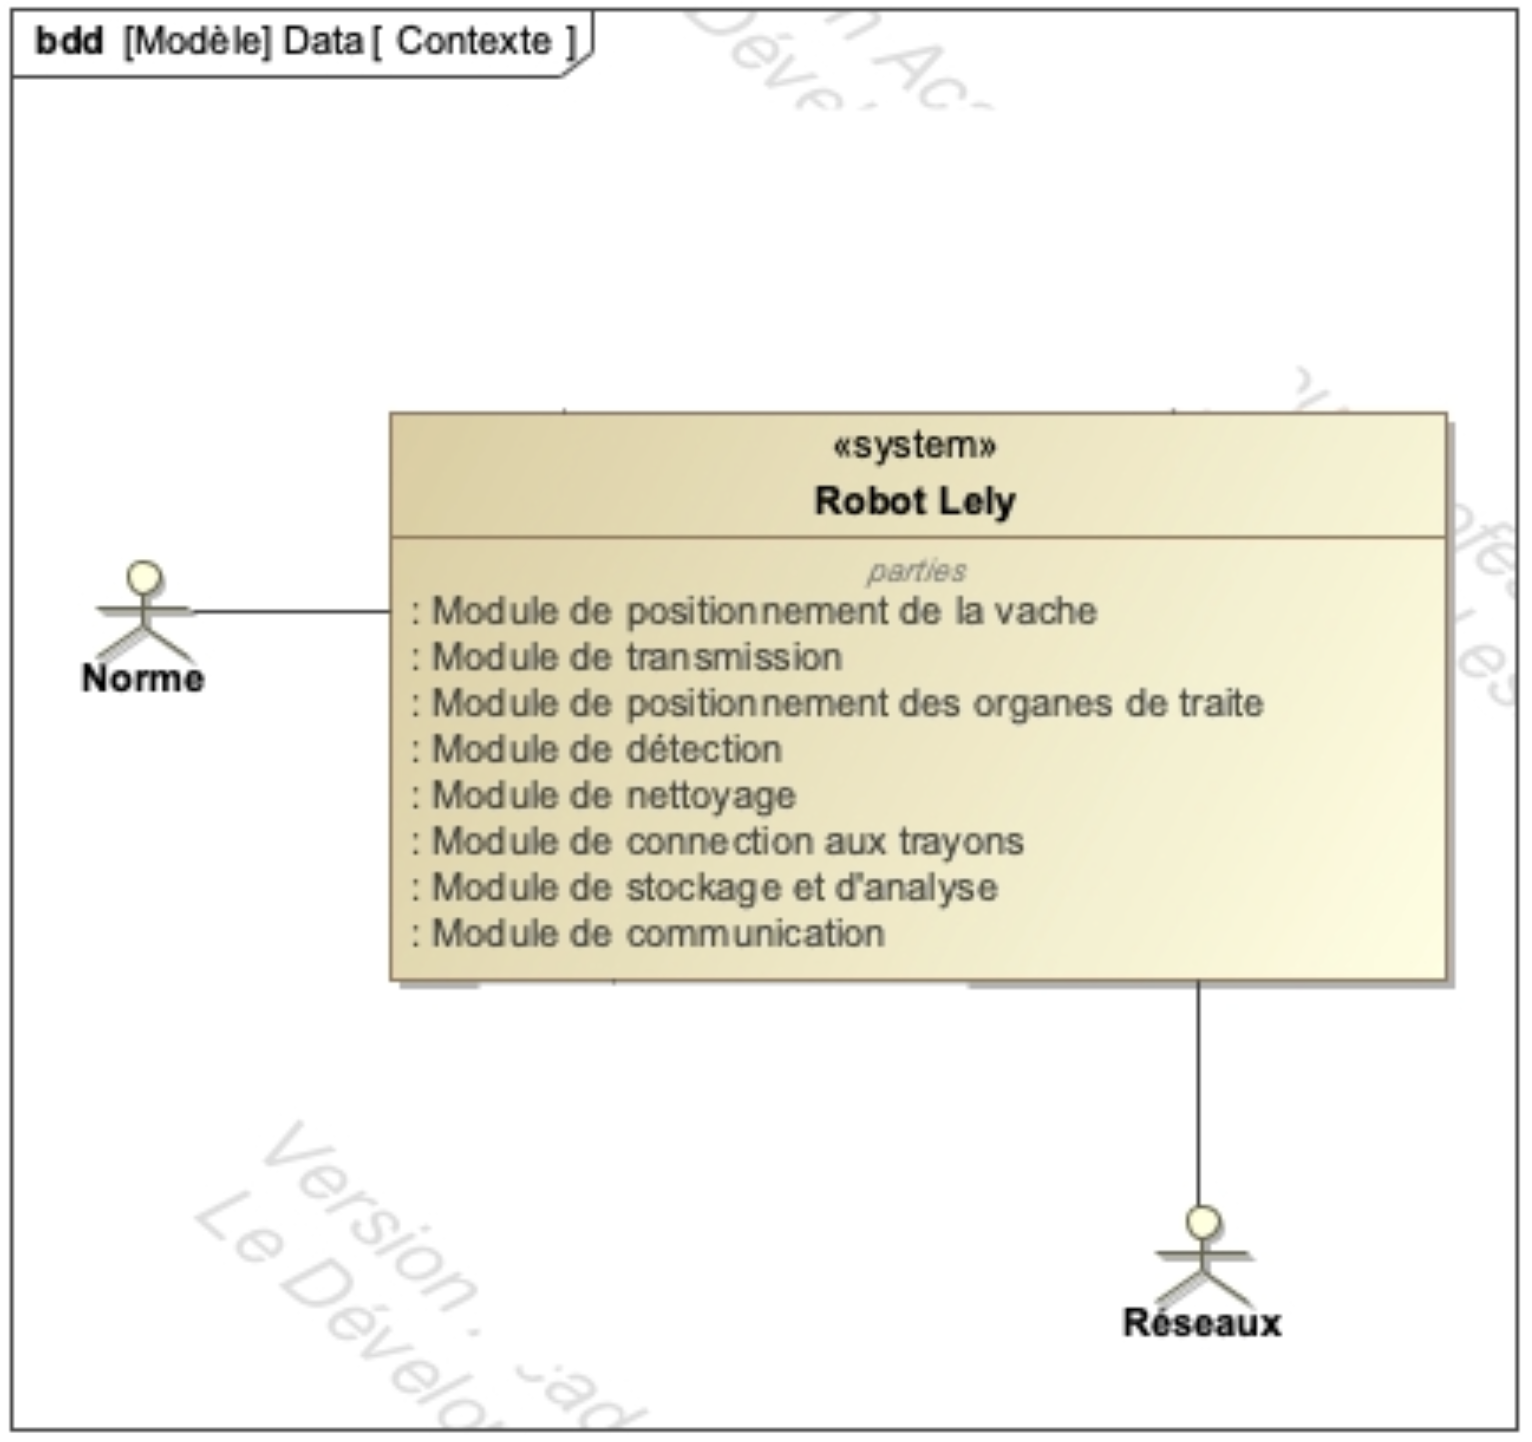
\includegraphics[width=0.6\linewidth]{img/contexte}
\end{center}}{\begin{center}
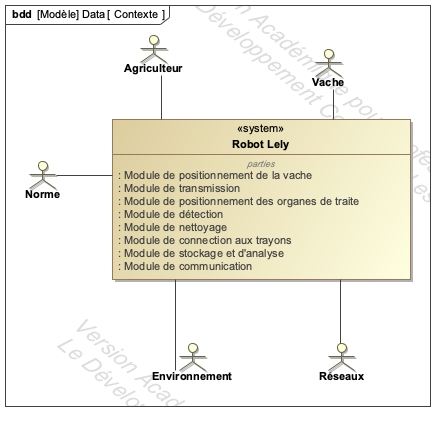
\includegraphics[width=0.6\linewidth]{img/contexte_cor}
\end{center}}

\reponse{4}{}{Exigences:
\begin{itemize}
 \item Traire les vaches,
 \item Alimenter les vaches.
\end{itemize}}

\reponse{4}{}{Le système de triangulation laser permet de positionner les gobelets trayeurs un par un.}

\reponse{4}{}{Lorsque la vache est dans le box, elle est installée sur un tapis de pesée équipé de capteurs de pesage.}

\reponse{4}{}{Toutes les vaches laitières du troupeau sont équipées d'un collier d'identification à infrarouge qu'elles portent autour du cou.}

\reponse{4}{}{$m_{tapis}=m_{revetement}+m_{structure}+m_{grille}=(2,5\cdot 1-0,7\cdot 0,5)\cdot 0,01\cdot 900+(2,5\cdot 1)\cdot 15=22,5+37,5+5,25=56,85$.

La masse d'une vache étant de 700kg, le tapis représente 8\% de la masse ce qui ne le rend pas négligeable.}

\reponse{4}{}{
\begin{eqnarray}
U_m(p)=r\cdot I_m(p)+L\cdot p\cdot I_m(p)+E(p) \nonumber \\
E(p)=K_e\cdot \Omega_m(p) \nonumber \\
Cm(p)=K_i\cdot I_m(p)  \nonumber \\
J\cdot p\cdot \Omega_m(p)=Cm(p)-\mu\cdot \Omega_m(p) \nonumber
\end{eqnarray}
}

\reponse{6}{}{
$U_m(p)=(r+L\cdot p)\cdot \frac{Cm(p)}{K_i}+K_e\cdot \Omega_m(p)$

$U_m(p)=(r+L\cdot p)\cdot \frac{(J\cdot p+\mu)\cdot \Omega_m(p)}{K_i}+K_e\cdot \Omega_m(p)$

Donc $H(p)=\frac{\Omega_m(p)}{U_m(p)}=\frac{K_i}{(r+L\cdot p)\cdot (J\cdot p+\mu)+K_e\cdot K_i}$
}

\reponse{1}{}{
Sous la forme canonique, on obtient:

$H(p)=\frac{\frac{K_i}{r\cdot \mu+K_e\cdot K_i}}{1+\frac{r\cdot J+L\cdot \mu}{r\cdot \mu+K_e\cdot K_i}\cdot p+\frac{L\cdot J}{r\cdot \mu+K_e\cdot K_i}\cdot p^2}$

La fonction de transfert est d'ordre 2 et de classe 0.
}

\reponse{3}{}{
$z=\frac{r\cdot J+L\cdot \mu}{2\cdot\sqrt{(r\cdot \mu+K_e\cdot K_i)\cdot L\cdot J}}$

$\omega_n=\sqrt{\frac{r\cdot \mu+K_e\cdot K_i}{L\cdot J}}$

$G=\frac{K_i}{r\cdot \mu+K_e\cdot K_i}$
}

\reponse{3}{}{
$G$ est en $V^{-1}\cdot rad\cdot s^{-1}=A.N^{-1}.m^{-1}=A.kg^{-1}.m^{-2}.s^2$

$G=1.52V^{-1}\cdot rad\cdot s^{-1}$.
}

\reponse{3}{}{
$w_n=100.4rad.s^{-1}$ et $z=4.7$
}

\reponse{3}{}{
$z>1$, cela signifie que les deux racines sont réelles.

$\tau_1.\tau_2=\frac{1}{w_n^2}$
$\tau_1+\tau_2=\frac{2.z}{w_n}$

$\tau_1^2+\tau_1.\tau_2-\frac{2.z}{w_n}.\tau_1=0$

$\tau_1^2+\frac{1}{w_n^2}-\frac{2.z}{w_n}.\tau_1=0$

$\tau_1^2+10^{-4}-0,1.\tau_1=0$

$\Delta=10^{-2}-4*10^{-4}=10^{-2}.(1-4*10^{-2})$

$\tau=\frac{0,1\pm 0,1\sqrt{1-4*10^{-2}}}{2}=\frac{0,1.(1\pm 0,98)}{2}$

$\tau_1=0,1s$ et $\tau_2=1ms$.
}

\reponse{3}{}{
$\tau_1>\tau_2$, cela signifie qu'une des deux racines est négligeable devant l'autre.

On peut alors écrire la fonction de transfert:
$H(p)=\frac{1}{1+0.005\cdot p}$
}

\reponse{3}{}{
$\omega_m(t)=u_0.(1-e^{\frac{-t}{\tau}})=25.(1-e^{\frac{-t}{0.005}})$
}

\reponse{3}{}{
Il s'agit de la courbe \ref{fig008b}, elle correspond bien à un premier ordre dont al constante de temps est $\tau=0.005s$, l'autre a un temps de réponse $\tau=0.015s$.}

\reponse{3}{}{$K.u_0=144$ avec $u_0=12$, donc $K=12$}

\reponse{3}{}{On sait que $(1+5\%).144=144+7.2=151.2$, ce qui ressemble au dépassement de la courbe, on en déduit que $\xi=0.69$.}


\reponse{3}{}{On sait que $t_{R5\%}.\omega_0=0.3$, or $t_{R5\%}=0.015s$ (graphiquement), donc $\omega_0=\frac{3}{0.015}=200rad.s^{-1}$}

\end{document}
